\documentclass{article}
\usepackage{arxiv}
\usepackage{graphicx}
\usepackage{amsmath,amssymb}
\usepackage{hyperref}
\usepackage{multicol}
\usepackage[numbers]{natbib}
\begin{document}
\title{Review Paper}
\author{Artificial Intelligence}
\date{\today}
\maketitle
\noindent
\twocolumn

\section*{Abstract}
Convolutional Neural Networks (CNNs) have become a cornerstone of deep learning for image analysis, demonstrating effectiveness in various tasks such as image classification, object detection, and semantic segmentation by learning spatial features through convolutional layers. Challenges persist regarding computational efficiency and adaptability to varying data complexities. While techniques like Neural Architecture Search (NAS) address these challenges, they often entail significant resource consumption. To mitigate these limitations, Self Expanding Neural Networks (SENN), inspired by neurogenesis, dynamically adjust network architecture during training, offering a promising avenue for adaptable and efficient models. This work introduces a Self Expanding Convolutional Neural Network (SECNN), extending the SENN concept to CNNs for vision tasks. The SECNN dynamically determines the optimal model size based on the task, eliminating the need for extensive architecture search and retraining, thereby enhancing efficiency and adaptability. Experimental results demonstrate the potential of feedforward trained CNNs, achieving competitive performance with backpropagation, particularly in neuromorphic hardware and unsupervised learning contexts, further expanding the understanding of neuronal information processing.


\section*{Introduction}
Convolutional Neural Networks (CNNs) have significantly advanced the field of deep learning, particularly in processing grid-like data such as images, demonstrating effectiveness in tasks including image classification, object detection, and semantic segmentation. This success stems from their ability to learn spatial features through convolutional layers that capture local patterns using shared weights implemented by kernels. Pooling layers further enhance this process by reducing spatial dimensions, enabling the network to focus on significant aspects.

Despite their widespread adoption, CNNs face challenges related to computational efficiency and adaptability. While architectures like MobileNet and EfficientNet have addressed efficiency, traditional CNNs with fixed architectures may not perform consistently across diverse input data with varying complexities. Neural Architecture Search (NAS) has emerged as a method for optimizing neural network architectures, but it is often resource-intensive, demanding substantial computational power and energy. This highlights the need for adaptable and efficient architectures that avoid over-parameterization.

To address these limitations, this research investigates Self Expanding Convolutional Neural Networks (SECNNs), extending the concept of Self Expanding Neural Networks (SENN) initially applied to multilayer perceptrons. The objective is to develop a SECNN that dynamically adjusts its model size based on the task at hand, thus enhancing efficiency. This approach eliminates the need for training multiple CNN models of varying sizes and avoids restarting the training process after model expansion, representing a significant step toward adaptable and efficient CNN models for various vision-related tasks.


\section*{Litrature Review}
Multi-column deep neural networks have been developed for image classification, as shown by Ciresan et al. \cite{1}. Their work highlights the effectiveness of utilizing multiple columns in the network architecture to enhance image classification performance. Further contributions by Ciresan et al. explored the application of deep neural networks for mitosis detection in breast cancer histology images \cite{2}. Their approach demonstrated the potential of deep learning in medical image analysis. Ciresan et al. also presented flexible, high-performance convolutional neural networks (CNNs) designed for image classification tasks \cite{3}. Additionally, Ciresan et al. introduced convolutional neural network committees for handwritten character classification \cite{4}. Their findings indicated the benefits of using committees of CNNs to improve classification accuracy.

The review by Egmont-Petersen et al. \cite{5} provides an overview of image processing techniques using neural networks, offering a comprehensive perspective on the role of neural networks in this domain. Furthermore, Farabet et al. \cite{6} explored hardware-accelerated convolutional neural networks for synthetic vision systems. Their research emphasizes the importance of hardware optimization for efficient CNN implementation.

Hinton provided a practical guide to training restricted Boltzmann machines \cite{7} and, with his colleagues, introduced a method for improving neural networks by preventing co-adaptation of feature detectors \cite{8}. This work addresses the issue of overfitting in neural networks.

The application of 3D convolutional neural networks for human action recognition was investigated by Ji et al. \cite{9}. Their study demonstrates the applicability of CNNs to video data for action recognition tasks. Similarly, Karpathy et al. \cite{10} presented a large-scale video classification approach using convolutional neural networks. Their research underscores the scalability of CNNs for complex video analysis.

Krizhevsky et al. \cite{11} achieved significant results in ImageNet classification using deep convolutional neural networks, showcasing the power of deep learning in large-scale image recognition. LeCun et al. \cite{12} demonstrated backpropagation for handwritten zip code recognition, a foundational work in applying neural networks to document recognition. LeCun et al. also applied gradient-based learning to document recognition \cite{13}.

Nebauer evaluated convolutional neural networks for visual recognition, providing insights into their performance and limitations \cite{14}. Best practices for CNNs applied to visual document analysis were presented by Simard et al. \cite{15}. Srivastava explored improving neural networks with dropout \cite{16}, a regularization technique.

Szarvas et al. \cite{17} used convolutional neural networks for pedestrian detection, highlighting their utility in object detection tasks. Furthering this, Szegedy et al. \cite{18} developed deep neural networks for object detection. Tivive and Bouzerdoum \cite{19} introduced a new class of convolutional neural networks (SiConNets) and applied them to face detection.

Zeiler and Fergus \cite{20} explored stochastic pooling for regularization of deep convolutional neural networks. Additionally, Zeiler and Fergus \cite{21} focused on visualizing and understanding convolutional networks, offering insights into their internal workings.

Andén and Mallat introduced the concept of deep scattering spectrum \cite{22}. Bruna and Mallat explored invariant scattering convolution networks \cite{23}, and Mallat \cite{28} discussed group invariant scattering. Mallat also provided insights into understanding deep convolutional networks \cite{29}. Furthermore, Bruna Estrach worked on Scattering representations for recognition \cite{25}.

Cortes and Vapnik introduced support-vector networks \cite{24}, and Kaiser Gerald presented "A friendly guide to wavelets" \cite{26}. LeCun et al. worked on Handwritten digit recognition with a back-propagation network \cite{27}.

LeCun, Bengio, and Hinton \cite{30} provided a comprehensive overview of deep learning, summarizing recent advances and future directions in the field.


\section*{Methodology}
Convolutional Neural Networks (CNNs) are utilized as a form of artificial neural network that leverages knowledge of specific input types to simplify network architecture, particularly in image analysis tasks. This approach shifts the focus from the entirety of the problem domain to specific, relevant features. Methodologically, the use of CNNs involves structuring the network with layers designed to exploit the properties of image data. One research direction explores a simplified model, such as the scattering transform based on wavelet transforms, to analyze CNN operations. The wavelet transform separates variations at different scales, contributing to feature transformation. Dynamically expanding CNN architectures can be developed, guided by an expansion criterion, such as a natural expansion score, to trigger model expansion. The research also involves labeling positive and negative data sets, crucial for training and evaluating the CNN model.


\section*{Convolutional Neural Networks (CNNs)}
CNNs are biologically inspired neural networks that use convolutional filters and non-linearities to solve problems. Their architecture is designed to process image data effectively by organizing neurons into three dimensions: height, width, and depth. Unlike standard ANNs, neurons in a CNN layer connect only to a small region of the preceding layer.

\subsection*{Convolutional Layer}
The convolutional layer is central to CNN operation, utilizing learnable kernels to convolve across the input's spatial dimensions, generating 2D activation maps. These kernels detect specific features at spatial positions. Each kernel has a corresponding activation map, and the output volume's depth is set by the number of neurons. To mitigate the size of models from training ANNs on images, each convolutional neuron connects to a small region of the input volume, known as the receptive field.

The complexity of the model is reduced via hyperparameters such as depth, stride, and zero-padding. The output's spatial dimensionality can be calculated using the formula:

$$(V - R) + 2Z \\over S + 1$$

where $V$ is the input volume size, $R$ is the receptive field size, $Z$ is the zero-padding, and $S$ is the stride.

Parameter sharing further reduces the number of parameters by constraining each activation map to the same weights and bias, which is based on the assumption that a region feature useful in one spatial location is likely to be useful in another.

\subsection*{CNN Architecture}
CNN architecture focuses on processing image-based inputs, organizing neurons in layers across three dimensions: spatial dimensionality (height and width) and depth. The depth signifies the third dimension of an activation volume. The input 'volume' will have a dimensionality of height $\\times$ width $\\times$ depth, leading to a final output layer comprised of a dimensionality of $1 \\times 1 \\times n$, where $n$ represents the possible number of classes.

\subsection*{Convolutional Neural Networks}
CNNs compute each subsequent layer $x_j$ as:

$$x_j = \u03c1W_jx_{j-1}$$

where $W_j$ is a linear operator (typically a convolution), and $\u03c1$ is a non-linearity (e.g., rectifier or sigmoid). The layers are filter maps and each layer can be written as a sum of convolutions of the previous layer:

$$x_j(u, k_j) = \u03c1(\\sum_k (x_{j-1}(., k) * W_{j,k_j}(., k))(u))$$

Here $*$ is the discrete convolution operator:

$$(f * g)(x) = \\sum_{u=-\\infty}^{\\infty} f(u)g(x - u)$$

The weights $W_j$ are learned by stochastic gradient descent using backpropagation.

\subsection*{General Convolutional Neural Network Architectures}
General CNN architectures extend the analysis of single-channel convolutions to allow for channel combinations, using tools developed by Mallat. This extension involves replacing contractions and invariants to translations by contractions along adaptive groups of local symmetries, and wavelets are replaced by adapted filter weights.

\subsection*{A Mathematical Framework for CNNs}
Mallat introduced a mathematical framework for analyzing CNNs based on wavelet scattering, illustrating that computing invariants requires separating variations of X at different scales with a wavelet transform.

\subsection*{Continuous Wavelet Transform}
The Continuous Wavelet Transform (CWT) captures variations in $f$ at a particular scale and provides a foundation for the operation of CNNs. It is defined as:

$$\\tilde{f}(s, t) \u2261 (f * \u03c8_s)(t)$$

where $*$ is the continuous convolution operator:

$$(p * q)(x) \u2261 \\int_{-\\infty}^{\\infty} p(u)q(x - u)du$$
and
$$\u03c8_s(u) \u2261 |s|^{-p}\u03c8(\\frac{u}{s})$$


\begin{figure}[h]
\centering
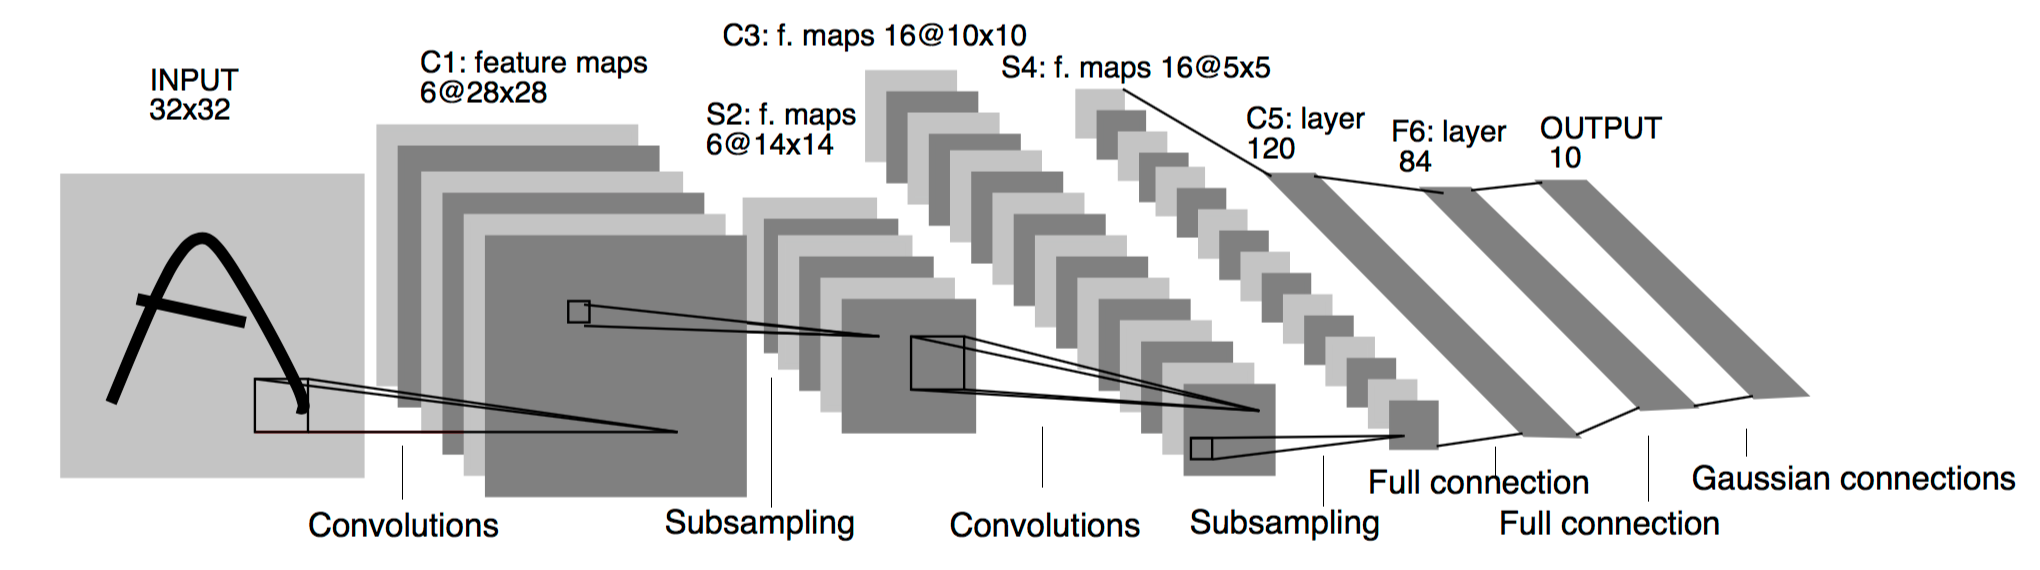
\includegraphics[width=0.9\linewidth]{C:/Users/VICKY/Desktop/New folder/output_directory/cnn2/image94-page3.png}
\end{figure}


\textbf{Figure Caption:} "Figure 1: Architecture of a Convolutional Neural Network, adapted from LeCun et al. \cite{7}, illustrating a standard layered structure for feature extraction and classification tasks."


\section*{Results}
The experiments conducted on CIFAR-10 image classification revealed notable performance metrics across multiple trials. Specifically, achieving 70% validation accuracy required approximately 11,360 parameters on average, while reaching 80% validation accuracy necessitated a significantly larger parameter count, averaging 33,655.2. The highest validation accuracy attained across these trials averaged 84.1%, achieved with a mean of 62,698.4 parameters. Furthermore, a methodology for implementing Class Activation Maps using FeedForward trained Convolutional Neural Networks (CNNs) was demonstrated, providing a tool for enhancing the explainability of AI models.


\section*{Conclusion}
Convolutional Neural Networks (CNNs) represent a cornerstone in deep learning-based image analysis, offering advantages over traditional methods through their capacity to exploit spatial information and facilitate explainable AI tools like class activation maps. The core innovation of CNNs lies in their ability to focus on specific input features, leading to simpler network architectures compared to other artificial neural networks. Research has strived to simplify and understand CNN operations, with approaches like the scattering transform providing insights into their feature transformation processes built upon wavelet transforms.

Recent advancements explore novel training methodologies, such as FeedForward (FF) trained CNNs, which demonstrate competitive performance relative to backpropagation with appropriate hyperparameter optimization. These techniques hold promise for addressing real-world computer vision challenges, particularly in neuromorphic hardware and unsupervised learning scenarios. Further research is needed to understand the individual and synergistic contributions of positive and negative labeling within FF training, and to explore its potential in training deeper networks and handling more complex datasets. Additionally, expanding on the work of Lorberbom et al. (2023) to better understand the ability of FF training to work with larger and more complex data sets needs to be explored.

Furthermore, dynamically expanding architectures, such as the Self Expanding Convolutional Neural Network, offer computationally efficient solutions for determining optimal architectures for vision tasks, eliminating the need for multiple training iterations. Future studies could focus on further optimization of these dynamically expanding architectures with more complex datasets. The connection to biological neuronal systems also remains a promising research avenue, potentially bridging the gap between artificial and biological intelligence.


\begin{thebibliography}{99}
\bibitem{1} Ciresan, D., Meier, U., Schmidhuber, J.: "Multi-column deep neural networks for image classification". In: Computer Vision and Pattern Recognition (CVPR), 2012 IEEE Conference on. pp. 3642–3649. IEEE (2012)

\bibitem{2} Cireșan, D.C., Giusti, A., Gambardella, L.M., Schmidhuber, J.: "Mitosis detection in breast cancer histology images with deep neural networks". In: Medical Image Computing and Computer-Assisted Intervention–MICCAI 2013, pp. 411–418. Springer (2013)

\bibitem{3} Ciresan, D.C., Meier, U., Masci, J., Maria Gambardella, L., Schmidhuber, J.: "Flexible, high performance convolutional neural networks for image classification". In: IJCAI Proceedings-International Joint Conference on Artificial Intelligence. vol. 22, p. 1237 (2011)

\bibitem{4} Cireșan, D.C., Meier, U., Gambardella, L.M., Schmidhuber, J.: "Convolutional neural network committees for handwritten character classification". In: Document Analysis and Recognition (ICDAR), 2011 International Conference on. pp. 1135–1139. IEEE (2011)

\bibitem{5} Egmont-Petersen, M., de Ridder, D., Handels, H.: "Image processing with neural networks a review". Pattern recognition 35(10), 2279–2301 (2002)

\bibitem{6} Farabet, C., Martini, B., Akselrod, P., Talay, S., LeCun, Y., Culurciello, E.: "Hardware accelerated convolutional neural networks for synthetic vision systems". In: Circuits and Systems (ISCAS), Proceedings of 2010 IEEE International Symposium on. pp. 257–260. IEEE (2010)

\bibitem{7} Hinton, G.: "A practical guide to training restricted boltzmann machines". Momentum 9(1), 926 (2010)

\bibitem{8} Hinton, G.E., Srivastava, N., Krizhevsky, A., Sutskever, I., Salakhutdinov, R.R.: "Improving neural networks by preventing co-adaptation of feature detectors". arXiv preprint arXiv:1207.0580 (2012)

\bibitem{9} Ji, S., Xu, W., Yang, M., Yu, K.: "3d convolutional neural networks for human action recognition". Pattern Analysis and Machine Intelligence, IEEE Transactions on 35(1), 221–231 (2013)

\bibitem{10} Karpathy, A., Toderici, G., Shetty, S., Leung, T., Sukthankar, R., Fei-Fei, L.: "Large-scale video classification with convolutional neural networks". In: Computer Vision and Pattern Recognition (CVPR), 2014 IEEE Conference on. pp. 1725–1732. IEEE (2014)

\bibitem{11} Krizhevsky, A., Sutskever, I., Hinton, G.E.: "Imagenet classification with deep convolutional neural networks". In: Advances in neural information processing systems. pp. 1097–1105 (2012)

\bibitem{12} LeCun, Y., Boser, B., Denker, J.S., Henderson, D., Howard, R.E., Hubbard, W., Jackel, L.D.: "Backpropagation applied to handwritten zip code recognition". Neural computation 1(4), 541–551 (1989)

\bibitem{13} LeCun, Y., Bottou, L., Bengio, Y., Haffner, P.: "Gradient-based learning applied to document recognition". Proceedings of the IEEE 86(11), 2278–2324 (1998)

\bibitem{14} Nebauer, C.: "Evaluation of convolutional neural networks for visual recognition". Neural Networks, IEEE Transactions on 9(4), 685–696 (1998)

\bibitem{15} Simard, P.Y., Steinkraus, D., Platt, J.C.: "Best practices for convolutional neural networks applied to visual document analysis". In: null. p. 958. IEEE (2003)

\bibitem{16} Srivastava, N.: "Improving neural networks with dropout". Ph.D. thesis, University of Toronto (2013)

\bibitem{17} Szarvas, M., Yoshizawa, A., Yamamoto, M., Ogata, J.: "Pedestrian detection with convolutional neural networks". In: Intelligent Vehicles Symposium, 2005. Proceedings. IEEE. pp. 224–229. IEEE (2005)

\bibitem{18} Szegedy, C., Toshev, A., Erhan, D.: "Deep neural networks for object detection". In: Advances in Neural Information Processing Systems. pp. 2553–2561 (2013)

\bibitem{19} Tivive, F.H.C., Bouzerdoum, A.: "A new class of convolutional neural networks (siconnets) and their application of face detection". In: Neural Networks, 2003. Proceedings of the International Joint Conference on. vol. 3, pp. 2157–2162. IEEE (2003)

\bibitem{20} Zeiler, M.D., Fergus, R.: "Stochastic pooling for regularization of deep convolutional neural networks". arXiv preprint arXiv:1301.3557 (2013)

\bibitem{21} Zeiler, M.D., Fergus, R.: "Visualizing and understanding convolutional networks". In: Computer Vision–ECCV 2014, pp. 818–833. Springer (2014)

\bibitem{22} Andén, J., Mallat, S.: "Deep scattering spectrum". Signal Processing, IEEE Transactions on, 62(16):4114–4128, 2014.

\bibitem{23} Bruna, J., Mallat, S.: "Invariant scattering convolution networks". Pattern Analysis and Machine Intelligence, IEEE Transactions on, 35(8):1872–1886, 2013.

\bibitem{24} Cortes, C., Vapnik, V.: "Support-vector networks". Machine learning, 20(3): 273–297, 1995.

\bibitem{25} Bruna Estrach, J.: "Scattering representations for recognition".

\bibitem{26} Kaiser Gerald.: "A friendly guide to wavelets", 1994.

\bibitem{27} Boser Le Cun, B, Denker, J.S., Henderson, D., Howard, R.E., Hubbard, W., Jackel, L.D.: "Handwritten digit recognition with a back-propagation network". In Advances in neural information processing systems. Citeseer, 1990.

\bibitem{28} Mallat, S.: "Group invariant scattering". Communications on Pure and Applied Mathematics, 65(10):1331–1398, 2012.

\bibitem{29} Mallat, S.: "Understanding deep convolutional networks". arXiv preprint arXiv:1601.04920, 2016.

\bibitem{30} Yann LeCun, Yoshua Bengio, and Geoffrey Hinton. "Deep learning". Nature, 521(7553):436–444, 2015.
\end{thebibliography}

\end{document}
